%!TEX root = apunte_estadistica.tex


\chapter{Inferencia bayesiana}


El enfoque que hemos revisado hasta ahora  es el clásico o \emph{frecuentista}, este punto de vista asume lo siguiente: 
\begin{itemize}
	\item El concepto de probabilidad está relacionado con frecuencias límites, es decir, la probabilidad de un evento es la razón de veces que este ocurre versus las veces que no ocurre (usualmente referido como \emph{casos favorables dividido por casos totales}). En este sentido, la probabilidad es una propiedad del mundo real. 
	\item Los parámetros son constantes (fijos) y desconocidos, es decir, no existe \emph{aleatoriedad} relacionada a los parámetros, por ende no podemos construir enunciados probabilísticos con respecto a ellos
	\item El procedimiento estadístico debe comportarse bien en el largo plazo, un ejemplo de esto es que un ($1-\alpha$)-intervalo de confianza debe capturar (asintóticamente) el parámetro una fracción $1-\alpha$ de las veces luego de infinitos experimentos. 
\end{itemize}

En este capítulo consideraremos un enfoque alternativo al análisis estadístico, el cual llamaremos \textbf{enfoque bayesiano}, y que se caracteriza por lo siguiente: 

\begin{itemize}
 	\item La probabilidad es subjetiva y denota un grado de \emph{creencia}, es decir, la aleatoriedad de un evento no solo es intrínseca de éste sino también de nuestra observación
 	\item Lo anterior permite considerar aleatoriedad en los parámetros, pues el hecho de que éstos sean fijos no quiere decir que los conozcamos. 
 	\item Podemos considerar los parámetros como VAs y, consecuentemente, calcular su distribución de probabilidad. Inferencias puntuales o la incidencia de este parámetro en otras VAs está completamente determinada por su distribución.
 \end{itemize}

 Existen ventajas y desventajas para ambos enfoques, lo cual hace que ambos sean considerados en distintas aplicaciones. Si bien el enfoque bayesiano es muy antiguo, la estadística clásica ha privilegiado un punto de vista frecuentista, mientras que disciplinas como minería de datos y aprendizaje de máquinas se inclinan por el enfoque bayesiano. De todas formas actualmente ambos métodos se consideran en base a sus propios méritos, entonces, dejando materias filosóficas de lado nos dedicaremos a estudiar como se hace inferencia bayesiana. 

\clase{clase 18: 10/10}
 \section{Distribuciones a priori y a posteriori} 
 \label{sec:distribuciones_a_priori_y_a_posteriori}
 
Consideraremos que tanto el parámetro $\theta$ y la cantidad de interés $X$ son VAs. En este sentido, definiremos la distribución del parámetro como $p(\theta)$ y la distribución de $X$ condicional al parámetro como $p(X|\theta)$. Observemos que ya no usamos la notación $p_\theta(X)$, pues damos énfasis en que $\theta$ es una VA. Nos referiremos a $p(\theta)$ como la distribución \textbf{a priori} sobre $\theta$, o simplemente el prior sobre $\theta$. Formalmente, re-definamos el concepto de \textit{familia paramétrica}. 

\begin{definition}
	\label{def:fam_par_bayes}
	Sea $(S,\cA,\mu)$ un espacio de probabilidad y sean $(\cX,\cB)$ y $(\Omega, \tau)$ espacios borelianos. Sean $X:S\to\cX$ y  $\Theta:S\to\Omega$ funciones medibles, entonces, $\Theta$ se llama parámetro y $\Omega$ se llama espacio de parámetros. La distribución condicional $X$ dado $\Theta$ se llama familia paramétrica de distribuciones de $X$ y está denotada por 
	\begin{equation}
		\cP = \{P_\theta \tq \forall A\in\cB, P_\theta(A) = \Prob{X\in A |  \Theta=\theta}, \theta\in\Omega\}
	\end{equation}. 
\end{definition}

Observemos que la definición de familia paramétrica en el contexto bayesiano solo dice relación con las distribuciones condicionales $\Prob{X|\theta}$ que denota la distribución de $X$ una vez que $\Theta=\theta$ ha sido observado. Sin embargo, el contexto también permite identificar la distribución \textit{a priori} de $\Theta$, $\mu_\Theta$, la cual es una medida en $(\Omega,\tau)$ inducida por $\Theta$ desde $\mu$. 


Asumiremos que $P_\theta$ como medida en $(\cX,\cB)$ tiene densidad (con respecto a alguna medida $\nu$) dada por
\begin{equation}
 	p_\theta(x|\theta) = \frac{dP_\theta}{d\nu}(x).
 \end{equation}
 Asumiremos que $p_\theta(x|\theta)$ es medible con respecto a la sigma-álgebra producto, lo cual permitirá integrarla tanto en $x\in\cX$ como en $\theta\in\Omega$. Esto nos permite verificar que la densidad condicional de $X$ dado $\theta$ con respecto a $\nu$ cumple con 
 \begin{equation}
  	\Prob{X\in A |\Theta=\theta } = \int_A p(x|\theta)\d\nu(x),\ A\in\cB.
  \end{equation} 
  Adicionalmente, podemos notar que la distribución \textbf{marginal} de X puede ser calculada integrando la distribución condicional con en todo el espacio de parámetros: Para $A\in\cB$ tenemos
  \begin{align}
  	\mu_X(A) &= \int_\Omega \left(\int_A p(x|\theta)\d\nu(x)\right)\d\mu_\Theta(\theta)\\
  			&= \int_A \int_\Omega  p(x|\theta) \d\mu_\Theta(\theta) \d\nu(x)\nonumber
  \end{align}
  lo cual implica directamente que $\mu_X(A)$ es absolutamente contínua c.r.a. $\nu$ también con densidad 
  \begin{equation}
  	p(x) = \int_\Omega  p(x|\theta) \d\mu_\Theta(\theta)
  \end{equation}
  la cual conocemos como densidad marginal de $X$.

La distribución condicional de $\Theta$ dado $X=x$, denotada por $\mu_{\Theta|X}(\theta|x)$, es conocida como la distribución a posteriori o simplemente \textit{posterior}. El siguiente teorema es el elemento fundamental de la inferencia bayesiana, pues permite calcular la distribución posterior. 
\begin{theorem}[Bayes] Asumamos que $X$ sigue una familia paramétrica $\{P_\theta\}$ como en la Definición \ref{def:fam_par_bayes} y asumamos que $P_\theta\ll \nu ,\forall\theta\in\Omega$, para alguna medida $\nu$ en $(\cX,\cB)$. Denotemos 
\begin{itemize}
	\item  $p(x|\theta)$: la densidad (con respecto a $\nu$) de $X$ dado $\Theta = \theta$
	\item  $\mu_\Theta$: la distribución a priori de $\Theta$
	\item $\mu_{\Theta|X}(\cdot|x)$: la distribución condicional de $\Theta$ dado $X=x$.
\end{itemize} 

Entonces, $\mu_{\Theta|x} \ll \mu_\Theta$ c.s. con respecto a la ley marginal de X, $\mu_X$, y su derivada de Radon-Nikodym es

\begin{equation}
	\frac{d\mu_{\Theta|X}}{d\mu_\Theta} (\theta|x) = \frac{p(x|\theta)}{\int_\Omega p(x|t) \d\mu_\Theta(t)}
\end{equation}	
\end{theorem}
\todo[inline]{demostración está pendiente}
Con el resultado anterior, podemos verificar que para $T\in\Omega$ la posterior cumple 
\begin{align}
	\Prob{\Theta\in T} &= \int_C \frac{p(x|\theta)}{\int_\Omega p(x|t) \d\mu_\Theta(t)} d\mu_\Theta(\theta)\\
	&= \frac{1}{\int_\Omega p(x|t) \d\mu_\Theta(t)}\int_C p(x|\theta) d\mu_\Theta(\theta)
\end{align}


\begin{remark}[Prior absolutamente continuas]
Si bien no es necesario, asumamos que la distribución a priori $\mu_X$ es a.c. con respecto a la medida de Lebesgue, $\lambda$, y su densidad con respecto a dicha medida es
\begin{equation}
	p(\theta) = \frac{d\mu_\Theta}{d\lambda}(\theta).
\end{equation}
Entonces, como el teorema de Bayes establece que $\mu_{\Theta|x} \ll \mu_\Theta$ y nosotros hemos considerado $\mu_\Theta \ll  \lambda$, entonces tenemos que $\mu_{\Theta|x} \ll \lambda$ con densidad respecto a la medida de Lebesgue
\begin{equation}
 	p(\theta|x) = \frac{p(x|\theta)p(\theta)}{p(x)},
 \end{equation} 
	donde recordemos que $p(x) = \int_\Omega p(x|\theta)p(\theta)\d\theta$.
\end{remark}

\begin{example}[Posterior Gaussiana: varianza conocida]
	Consideremos la familia paramétrica $\cP  = \{\cN(\mu,\sigma^2), \sigma^2 \text{ conocido.}\}$ y el prior sobre $\mu$ dado por $\cN(\mu; \mu_0,\sigma_0^2)$. Dada una muestra $X_1,\ldots,X_n$ la  posterior está dada por 
	\begin{align}
		p(\theta|x) = \cN\left(\theta; \frac{1}{\frac{1}{\sigma^2_0}+\frac{n}{\sigma^2}}\left(\frac{\mu_0}{\sigma^2_0}+\frac{\sum_i^nx_i}{\sigma^2}\right),\left(\frac{1}{\sigma^2_0}+\frac{n}{\sigma^2}\right)^{-1}\right)
	\end{align}
\end{example}

\begin{example}[Posterior Bernoulli - prior uniforme]
	Consideremos las VAs $X_1,\ldots,X_n \sim\ber{\theta}$ con un prior uniforme sobre $\theta$. La posterior está dada por 
	\begin{equation}
	 	p(\theta) = \frac{\theta^{\sum X_i}(1-\theta)^{(n-\sum X_i)}\cdot1}{p(x)} 
	 \end{equation} 
	 lo cual podemos identificar como una distribución beta de parámetros $\alpha = \sum X_i + 1$ y $\beta = n-\sum X_i +1 $, es decir 
	 \begin{equation}
	 	p(\theta) = \frac{\Gamma{(\alpha)}\Gamma{(\beta)}}{\Gamma{(\alpha + \beta)}} \theta^{\alpha - 1}(1-\theta)^{\beta - 1}.
	 \end{equation} 
\end{example}

\begin{remark}
	 Observemos que no hemos calculado explícitamente la constante de normalización, esto es porque hemos calculado una versión proporcional de la posterior y luego hemos impuesto que su integral en todo $\Omega$ deber ser 1. Este procedimiento permite no solo una forma alternativa de calcular esta constante sino que muchas veces la única. 
\end{remark}

\clase{Clase 19: 15/10}

\begin{example}[Posterior Bernoulli - prior Beta]
	Consideremos las VAs $X_1,\ldots,X_n \sim\ber{\theta}$ pero ahora con un prior Beta dado por 
	\begin{equation}
		p(\theta) = \frac{\Gamma{(\alpha_0)}\Gamma{(\beta_0)}}{\Gamma{(\alpha_0 + \beta_0)}} \theta^{\alpha_0 - 1}(1-\theta_0)^{\beta_0 - 1}.
	\end{equation}
	Es este caso, la posterior está dada por 
	\begin{align}
	 	p(\theta) &= \frac{\Gamma{(\alpha_0)}\Gamma{(\beta_0)}}{\Gamma{(\alpha_0 + \beta_0)}} \frac{\theta^{\sum X_i}(1-\theta)^{(n-\sum X_i)} \theta^{\alpha_0 - 1}(1-\theta_0)^{\beta_0 - 1}}{p(x)} \\
	 	&= \frac{\Gamma{(\alpha_0)}\Gamma{(\beta_0)}}{p(x) \Gamma{(\alpha_0 + \beta_0)}} \theta^{\sum X_i + \alpha_0 - 1 }(1-\theta)^{(n-\sum X_i + \beta_0-1)} \\
	 	&= \bet{\sum X_i + \alpha_0, n-\sum X_i + \beta_0},
	 \end{align} 
	 lo cual podemos identificar como una distribución beta de parámetros $\alpha = \sum X_i + 1$ y $\beta = n-\sum X_i +1 $, es decir 
	 \begin{equation}
	 	p(\theta) = \frac{\Gamma{(\alpha)}\Gamma{(\beta)}}{\Gamma{(\alpha + \beta)}} \theta^{\alpha - 1}(1-\theta)^{\beta - 1}.
	 \end{equation}  
	 Consecuentemente, pasar del prior al posterior es simplemente actualizar los parámetros de la forma 
	 \begin{align}
	 	\alpha_0 &\to \sum X_i + \alpha_0\\
	 	\beta_0 &\to n-\sum X_i + \beta_0
	 \end{align}

\end{example}

Notemos que, para ciertas elecciones de distribuciones a priori la forma de la densidad posterior cambia y otras veces se mantiene (con respecto a la forma del prior). La siguiente definición caracteriza este fenómeno.

\begin{definition}[Prior conjugado] Sea un modelo con densidad $p(x|\theta)$ y un prior sobre $\theta$ con densidad $p(\theta)$. Decimos que $p(\theta)$ es conjugado con la verosimiltud $p(x|\theta)$ si la posterior 
\begin{equation}
	p(\theta|x) = \frac{p(x|\theta)p(\theta)}{p(x)}
\end{equation}
pertenece a la misma familia que el prior $p(\theta)$.
\end{definition}
El hecho que dos  distribuciones (i.e, prior y posterior) pertenezcan a la \textit{misma familia}, quiere decir que ambas tienen la misma forma funcional, e.g., $f_\lambda(\theta)$ pero con distintos valores para el \textit{parámetro} $\lambda$, el cual es un \textit{hiperparámetro} del modelo. 

\begin{example}[Distribución Multinomial]
Consideremos un VA multinomial $X\sim\mul{n,\theta}$ donde $\theta$ pertenece al simplex 
\begin{equation}
	\label{eq:simplex}
  \{\theta\in[0,1]^k:\theta_1 + \cdots + \theta_k = 1 \}.
 \end{equation} 
 La distribución multinomial genera vectores $X\in\N^k$ cuya $i-$ésima componente modela la cantidad de veces que ocurre el evento $i$ dentro de $k$ eventos en $n$ intentos. Por ejemplo, si lanzamos un dado balanceado 100 veces, el vector que contiene el conteo de veces que obtenemos cada cara puede modelarse como 
 \begin{equation}
  	\theta_\text{dado} \sim \mul{100,\left[\tfrac{1}{6},\tfrac{1}{6},\tfrac{1}{6},\tfrac{1}{6},\tfrac{1}{6},\tfrac{1}{6}\right]}.
  \end{equation} 
Denotando $X=[x_1,\ldots,x_n]$, observemos que una muestra multinomial $X\sim\mul{n,\theta}$ cumple con 
\begin{equation}
	\{x_i\}_{i=1}^k \subset \{0,1,\ldots,n\},\quad  \sum_{i=1}^kx_i = n.
\end{equation}

Finalmente, la distribución Multinomial está dada por 
\begin{equation}
 	\mul{X;n,\theta} = \frac{n!}{x_1!\cdots x_k!} \theta_1^{x_1}\cdots\theta_k^{x_k},
 \end{equation} 
 y es la generalización de 
\begin{itemize}
	\item Bernoulli cuando $k=2$ y $n=1$; pues $\ber{X;\theta} = \theta^{x} (1-\theta)^{1-x}$
	\item Categórica: cuando $n=1$; pues $\cat{X;\theta} = \theta_1^{x_1}\cdots\theta_k^{x_k}$
	\item Binomial: cuando $k=2$; pues $\bin{X;n,\theta} = \binom{n}{x} \theta^{x}(1-\theta)^{n-x}$
\end{itemize}
\end{example}

Observemos que el parámetro $\theta$ en la distribución multinomial (y las otras tres) es directamente la distribución discreta. Es decir, el construir un prior $p(\theta)$ implica definir una distribución sobre distribuciones discretas.  


\begin{definition}[Distribución de Dirichlet]
Consideremos la  distribución de Dirichlet
\begin{equation}
	\theta \sim \dir{\theta|\alpha} = \frac{1}{B(\alpha)} \prod_{i=1}^k \theta_i^{\alpha_i-1},
\end{equation}
donde $\alpha = (\alpha_1,\ldots,\alpha_k)$ es el parámetro de concentración y la constante de normalización está dada por $B(\alpha)=\prod_{i=1}^k\Gamma(\alpha_i)/\Gamma(\sum_{i=1}^k\alpha_i)$. El soporte de esta distribución es el simplex presentado en la ecuación \eqref{eq:simplex}.
\end{definition}
En el caso $k=3$, la distribución de Dirichlet puede ser graficada en el simplex de 2 dimensiones. La Figura \ref{fig:dist_Dirichlet} presenta tres gráficos para distintos valores del parámetro de concentración. 

\begin{figure}[h]
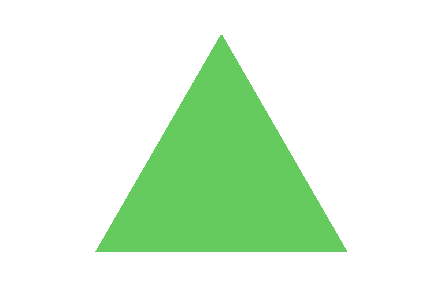
\includegraphics[width=0.3\textwidth]{img/dirichlet111.png}
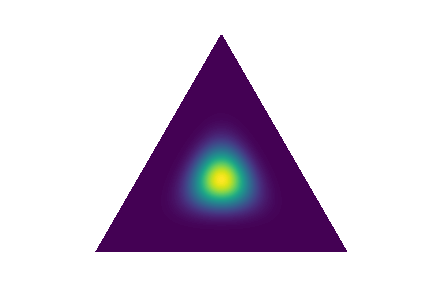
\includegraphics[width=0.3\textwidth]{img/dirichlet101010.png}
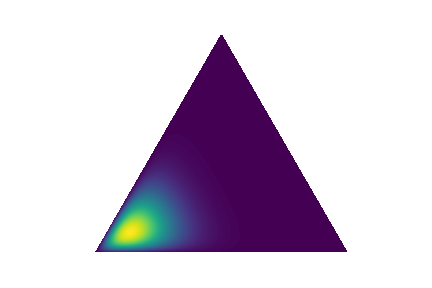
\includegraphics[width=0.3\textwidth]{img/dirichlet1022.png}
\caption{Distribuciones Dirichlet para $k=3$ con parámetros de concentración $\alpha$ (desde izquierda a derecha) dado por $[1,1,1]$, $[10,10,10]$ y $[10,2,2]$. }.
\label{fig:dist_Dirichlet}
\centering
\end{figure}


Veamos a continuación que la distribución de Dirichlet es conjugada al modelo Multinomial, y consecuentemente para Bernoulli, Categórica y Binomial. En efecto, si $\theta \sim \dir{\theta;\alpha}$ y $X\sim\mul{X;n,\theta}$, entonces

\begin{align}
	p(\theta|x) &= \frac{\mul{x;n,\theta}\dir{\theta;\alpha}}{p(x)}\nonumber\\
				&=  \frac{n!}{ x_1!\cdots x_k!p(x) B(\alpha)} \prod_{i=1}^k \theta_i^{x_i + \alpha_i-1}\nonumber\\
				&=  \frac{1}{B(\alpha')} \prod_{i=1}^k \theta_i^{\alpha'_i-1}
				\label{eq:dirichlet_post}
\end{align}
donde $\alpha' = (\alpha'_1,\ldots,\alpha'_k) = (\alpha'_1 + x_1,\ldots,\alpha'_k+ x_k)$ es el nuevo parámetro de concentración.

\begin{example}
	Consideremos $\alpha = [1,2,3,4,5]$ y generemos una muestra de $\theta\sim\dir{\theta|\alpha}$. El siguiente código genera, grafica e imprime esta muestra. 
	\begin{lstlisting}[language=Python]
	import numpy as np
	alpha = np.array([1,2,3,4,5]) 
	theta = np.random.dirichlet(alpha)
	plt.bar(np.arange(5)+1, theta);
	print(f'theta = {theta}')
\end{lstlisting}
En nuestro caso, obtuvimos los parámetros $ \theta = [0.034, 0.171, 0.286, 0.185, 0.324]$.

 Ahora, usaremos un prior Dirichlet sobre $\theta$ con $\alpha_p = [1,1,1,1,1]$ calcularemos la posterior de acuerdo a la ecuación \ref{eq:dirichlet_post}. La Figura \ref{fig:post_Dirichlet} muestra 100 muestras de la distribución posterior para una cantidad de observaciones igual a 






\begin{figure}[h]
\centering
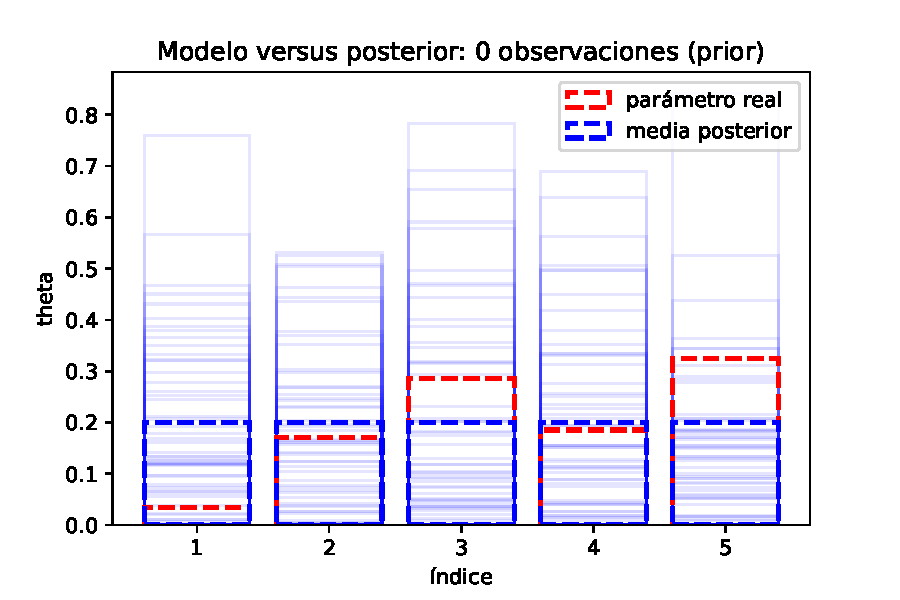
\includegraphics[width=0.3\textwidth]{img/post_dirichlet_0.pdf}
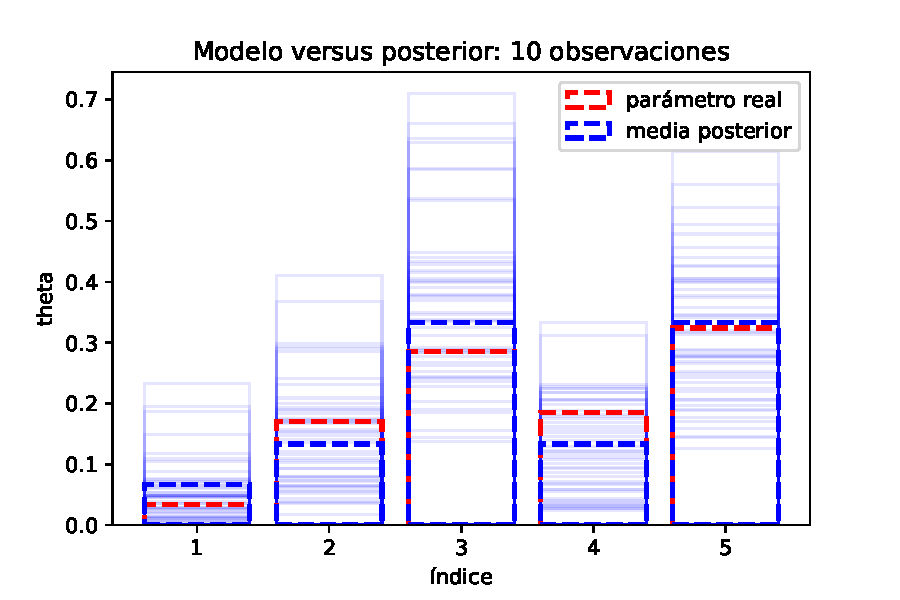
\includegraphics[width=0.3\textwidth]{img/post_dirichlet_10.pdf}
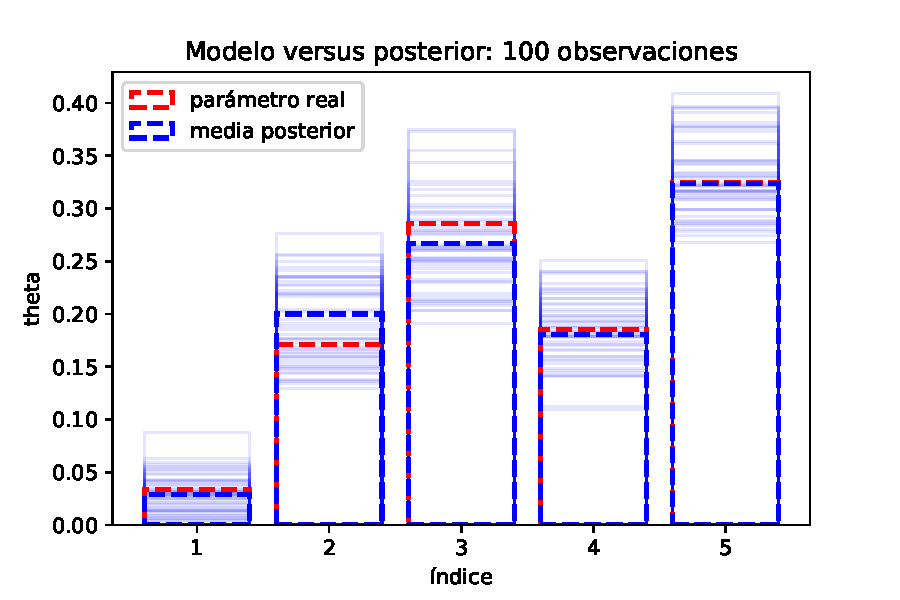
\includegraphics[width=0.3\textwidth]{img/post_dirichlet_100.pdf}\\
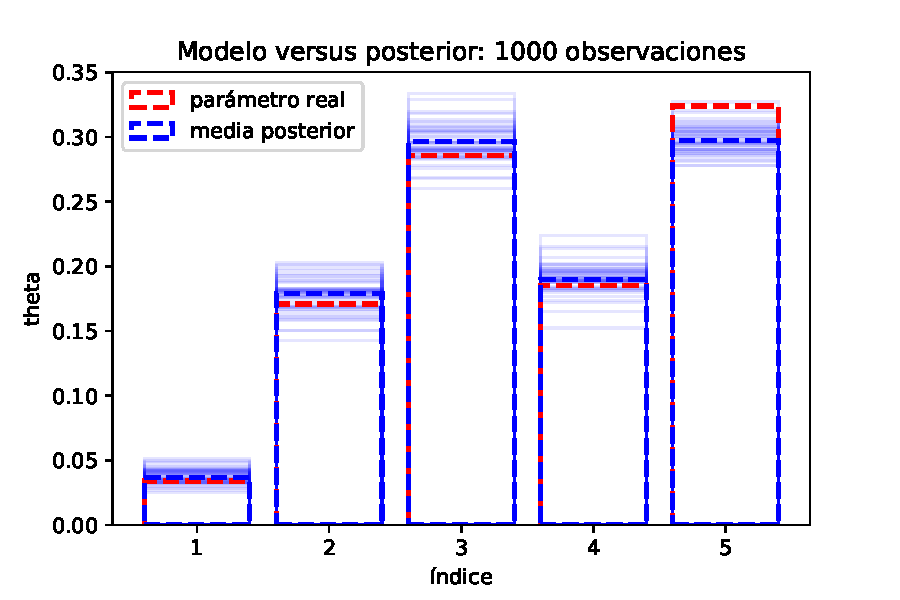
\includegraphics[width=0.3\textwidth]{img/post_dirichlet_1000.pdf}
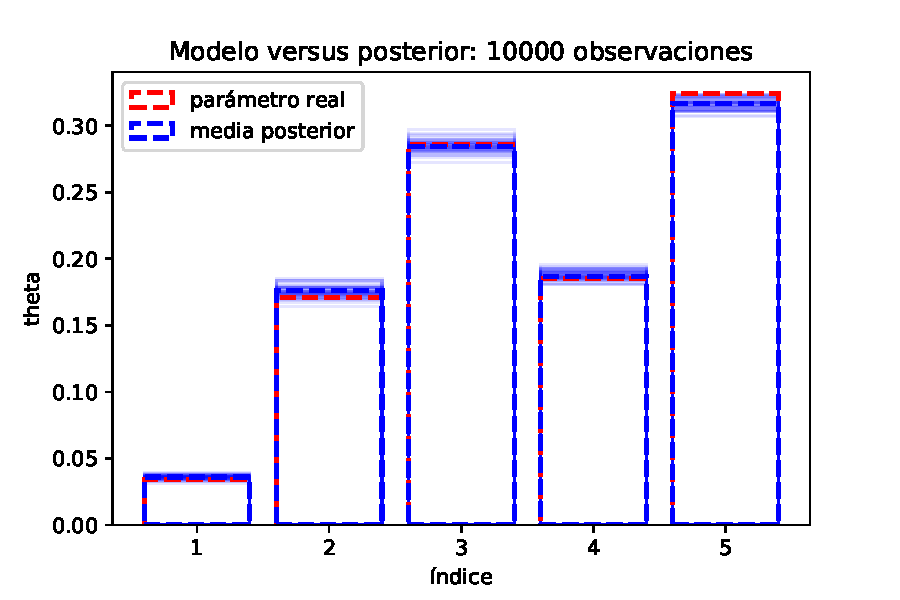
\includegraphics[width=0.3\textwidth]{img/post_dirichlet_10000.pdf}
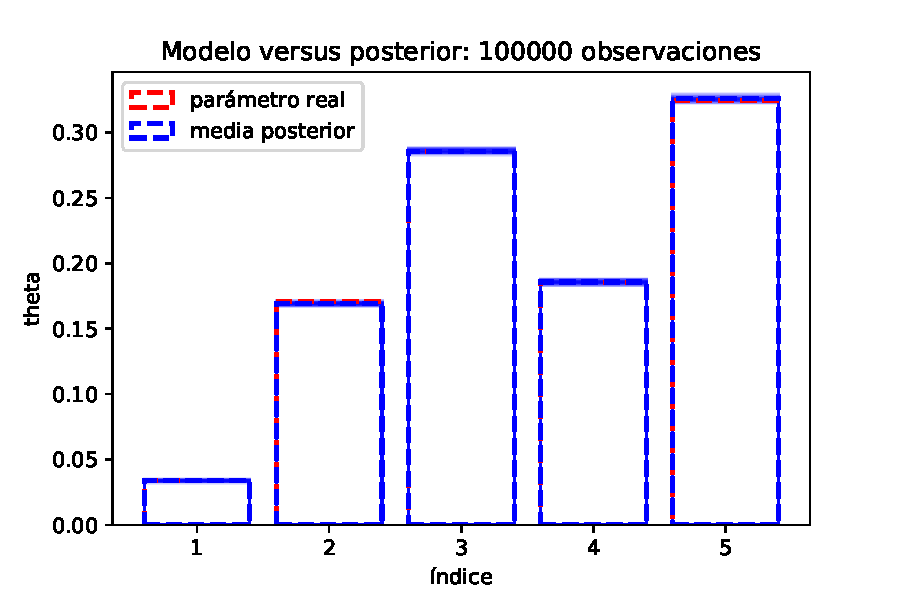
\includegraphics[width=0.3\textwidth]{img/post_dirichlet_100000.pdf}
\caption{Distribuciones Dirichlet para $k=3$ con parámetros de concentración $\alpha$ (desde izquierda a derecha) dado por $[1,1,1]$, $[10,10,10]$ y $[10,2,2]$. }.
\label{fig:post_Dirichlet}

\end{figure}


\end{example}

Los modelos y sus prior conjugados que hemos visto hasta ahora han pertenecido a la familia exponencial. En general, notemos que en el caso general si el modelo sigue una densidad de la familia exponencial, es decir
\begin{equation}
	p(x|\theta) = h_m(x)\expo{\theta^\top T(x)-A_m(\theta)},
\end{equation}
tiene un prior conjugado dado por 
\begin{equation}
	p(\theta|\lambda) = h_p(\theta)\expo{\lambda_1^\top \theta + \lambda_2^\top(-A_m(\theta)) -A_p(\lambda)}
\end{equation}
donde el parámetro natural $\lambda = [\lambda_1, \lambda_2]$ tiene dimensión $\text{dim}(\theta) +1 $ y el estadístico suficiente es $[\theta, -A_m(\theta)]$. El resto de los términos como $h_p$ y $A_p$ dependen de la forma particular de modelo. 

Calculando la distribución posterior tenemos que 

\begin{align}
	p(\theta|x_{1:n},\lambda) 
	&\propto \prod_{i=1}^np(x_i|\theta,\lambda)p(\theta|\lambda)\\
	&=\left(\prod_{i=1}^n h_m(x_i)\right) h_p(\theta) \expo{\theta^\top \sum_{i=1}^nT(x_i)-nA_m(\theta)+\lambda_1^\top \theta + \lambda_2^\top(-A_m(\theta)) -A_p(\lambda)}\nonumber\\
	&\propto h_p(\theta) \expo{\theta^\top \sum_{i=1}^nT(x_i)-nA_m(\theta)+\lambda_1^\top \theta + \lambda_2^\top(-A_m(\theta)) -A_p(\lambda)}\nonumber\\
	&\propto h_p(\theta) \expo{\left(\sum_{i=1}^nT(x_i)+\lambda_1\right)^\top\theta + (n+\lambda_2)(-A_m(\theta))}\nonumber
\end{align}


